\documentclass[aspectratio=169]{beamer}

% Shared Beamer settings for Applied Machine Learning lectures (UPES).
% Keep this file free of \documentclass to allow reuse via \input.

% Allow lecture sources to use shared theme/assets without copying them into each lecture folder.
% NOTE: These paths are relative to `Unit-xx/Lecture-yy/latex/` (and `Lab/Experiment-xx/latex/`).
\makeatletter
\def\input@path{{../../../_shared/}{../../../_shared/UPES-Beamer-Theme/}}
\makeatother

\usetheme{UPES}
\setbeamertemplate{navigation symbols}{}

\usepackage{amsmath}
\usepackage{amssymb}
\usepackage{booktabs}
\usepackage{graphicx}
\usepackage{hyperref}
\usepackage{xcolor}
\usepackage{listings}

% Code listings (Python-oriented for this subject).
\lstset{
  language=Python,
  basicstyle=\ttfamily\small,
  keywordstyle=\color{blue},
  commentstyle=\color{gray},
  stringstyle=\color{teal},
  showstringspaces=false,
  columns=fullflexible,
  breaklines=true
}

\usepackage{tikz}
\usetikzlibrary{arrows.meta,positioning,shapes.geometric,calc,fit,backgrounds}

% Per-slide source line (references shown on the slide itself).
\newcommand{\slidesources}[1]{%
  \vfill
  {\tiny\color{gray}\raggedright\sloppy\parbox{\linewidth}{Sources: #1}\par}%
}

% Unit-wise source strings for this subject (used by slides/notes).
% Path is relative to the lecture `latex/` folder (the compilation CWD).
% Source strings for Applied Machine Learning (CSAI2017P) — used by slides + notes.
% Prescribed texts and reference books are taken from the course syllabus.
% Support texts are the author-hosted open-access editions:
%   statlearning.com            (ISL with Python)
%   probml.github.io/pml-book   (Murphy, Probabilistic Machine Learning)
%   d2l.ai                      (Dive into Deep Learning)
%   mml-book.github.io          (Mathematics for Machine Learning)

\newcommand{\AMLRepoURL}{https://github.com/tali7c/Applied-Machine-Learning}

% --- prescribed -------------------------------------------------------------
\newcommand{\AMLPrescribed}{%
M\"uller and Guido, \textit{Introduction to Machine Learning with Python}, O'Reilly, 2016.;%
Bishop, \textit{Pattern Recognition and Machine Learning}, Springer, 2006.;%
Murphy, \textit{Machine Learning: A Probabilistic Perspective}, MIT Press, 2012.;%
Han, Kamber and Pei, \textit{Data Mining: Concepts and Techniques} (3e), Morgan Kaufmann, 2012.%
}

% --- unit-wise ---------------------------------------------------------------
\newcommand{\AMLUnitISources}{%
M\"uller and Guido, \textit{Introduction to Machine Learning with Python}, Ch. 1.;%
Bishop, \textit{Pattern Recognition and Machine Learning}, Ch. 1.;%
Murphy, \textit{Probabilistic Machine Learning: An Introduction}, MIT Press, 2022, Ch. 1.;%
Mitchell, \textit{Machine Learning}, McGraw Hill, 1997, Ch. 1.;%
Scikit-learn documentation, accessed 2026-08-04.%
}

\newcommand{\AMLUnitIISources}{%
Bishop, \textit{Pattern Recognition and Machine Learning}, \S1.5, \S4.3, \S7.1.;%
Zhang, Lipton, Li and Smola, \textit{Dive into Deep Learning}, \S3.4.;%
Shalev-Shwartz and Ben-David, \textit{Understanding Machine Learning}, Ch. 15.;%
Murphy, \textit{Probabilistic Machine Learning: An Introduction}, Ch. 5.%
}

\newcommand{\AMLUnitIIISources}{%
Zhang, Lipton, Li and Smola, \textit{Dive into Deep Learning}, Ch. 12 (Optimization Algorithms).;%
Deisenroth, Faisal and Ong, \textit{Mathematics for Machine Learning}, Ch. 7.;%
Kingma and Ba, ``Adam: A Method for Stochastic Optimization,'' ICLR 2015.;%
Ruder, ``An overview of gradient descent optimization algorithms,'' arXiv:1609.04747, 2016.%
}

\newcommand{\AMLUnitIVSources}{%
Han, Kamber and Pei, \textit{Data Mining: Concepts and Techniques} (3e), Ch. 3.;%
M\"uller and Guido, \textit{Introduction to Machine Learning with Python}, Ch. 3--4.;%
James, Witten, Hastie, Tibshirani and Taylor, \textit{An Introduction to Statistical Learning with Python}, Ch. 5--6, 12.;%
Scikit-learn documentation (preprocessing, model selection), accessed 2026-08-04.%
}

\newcommand{\AMLUnitVSources}{%
James et al., \textit{An Introduction to Statistical Learning with Python}, Ch. 3--6.;%
Bishop, \textit{Pattern Recognition and Machine Learning}, Ch. 3.;%
Deisenroth, Faisal and Ong, \textit{Mathematics for Machine Learning}, Ch. 9.;%
M\"uller and Guido, \textit{Introduction to Machine Learning with Python}, \S2.3.%
}

\newcommand{\AMLUnitVISources}{%
Han, Kamber and Pei, \textit{Data Mining: Concepts and Techniques} (3e), Ch. 8--9.;%
James et al., \textit{An Introduction to Statistical Learning with Python}, Ch. 8--9.;%
Bishop, \textit{Pattern Recognition and Machine Learning}, Ch. 4--5, 7, 14.;%
Zhang et al., \textit{Dive into Deep Learning}, Ch. 5.%
}

\newcommand{\AMLUnitVIISources}{%
Han, Kamber and Pei, \textit{Data Mining: Concepts and Techniques} (3e), Ch. 10.;%
James et al., \textit{An Introduction to Statistical Learning with Python}, Ch. 12.;%
M\"uller and Guido, \textit{Introduction to Machine Learning with Python}, \S3.5.;%
Ester, Kriegel, Sander and Xu, ``A density-based algorithm for discovering clusters (DBSCAN),'' KDD 1996.%
}

\newcommand{\AMLLabSources}{%
M\"uller and Guido, \textit{Introduction to Machine Learning with Python}, companion notebooks.;%
McKinney, \textit{Python for Data Analysis} (3e), O'Reilly, 2022.;%
Scikit-learn user guide, accessed 2026-08-04.;%
Matplotlib and Seaborn documentation, accessed 2026-08-04.%
}



\graphicspath{{../figures/}{../images/}{../../../_shared/}{../../../_shared/UPES-Beamer-Theme/}}

\title[Applied Machine Learning]{Applied Machine Learning}
\subtitle{Unit 06 -- Lecture 13: Classification Foundations and
          K-Nearest Neighbour}
\author{Tofik Ali}
\institute{School of Computer Science, UPES Dehradun}
\date{Autumn 2026}

% ---- a compact "output" block so code and its result sit together ----------
\lstdefinestyle{outblk}{
  basicstyle=\ttfamily\scriptsize\color{black!75},
  backgroundcolor=\color{black!5}, frame=leftline, framerule=2pt,
  rulecolor=\color{black!30}, breaklines=true, columns=fullflexible,
  keepspaces=true,   % several outputs below are aligned tables
  language={},       % printed output is not Python: do not syntax-highlight it
  xleftmargin=4pt, aboveskip=1pt, belowskip=1pt, literate={-}{{-}}1}
\lstnewenvironment{outblk}{\lstset{style=outblk}}{}

\begin{document}

\UPESCoverFrame
\setcounter{framenumber}{0}

\begin{frame}
  \titlepage
  \begin{center}
    \footnotesize The first classifier, and the one you can check with a
    pen\\[0.25em]
    \footnotesize Topic focus: \textbf{$k$-NN has no training step at
    all}\\[0.25em]
    \footnotesize Repository: \texttt{\AMLRepoURL}
  \end{center}
  \slidesources{\AMLUnitVISources}
\end{frame}

\begin{frame}{Quick Links}
  \centering
  \hyperlink{sec:setting}{\beamerbutton{The setting}}\hspace{0.4em}
  \hyperlink{sec:lazy}{\beamerbutton{Instance-based}}\hspace{0.4em}
  \hyperlink{sec:knn}{\beamerbutton{$k$-NN}}\hspace{0.4em}
  \hyperlink{sec:k}{\beamerbutton{Choosing $k$}}\hspace{0.4em}
  \hyperlink{sec:scale}{\beamerbutton{Scaling}}\hspace{0.4em}
  \hyperlink{sec:metric}{\beamerbutton{Metrics}}\hspace{0.4em}
  \hyperlink{sec:curse}{\beamerbutton{The curse}}\hspace{0.4em}
  \hyperlink{sec:practical}{\beamerbutton{Failure modes}}\hspace{0.4em}
  \hyperlink{sec:summary}{\beamerbutton{Summary}}
\end{frame}

\begin{frame}{Agenda}
  \tableofcontents
\end{frame}

\begin{frame}[shrink=6]{How this lecture works}
  \begin{columns}[T]
    \begin{column}{0.48\textwidth}
      \begin{block}{Every idea appears twice}
        \begin{enumerate}
          \item \textbf{By hand} --- seven points, one query, two patients,
            five neighbours. Small enough to check on paper, and small enough
            to appear in a test.
          \item \textbf{In code} --- the same arithmetic on real data, so you
            see that \texttt{KNeighborsClassifier} does exactly that and
            nothing magic.
        \end{enumerate}
      \end{block}
    \end{column}
    \begin{column}{0.48\textwidth}
      \begin{alertblock}{Commit before you look}
        Five slides ask you to predict a number before it is revealed. Write
        your guess down. Being wrong on paper is how the idea sticks.
      \end{alertblock}
    \end{column}
  \end{columns}
  \vspace{0.4em}
  \begin{center}
    \small Two numbers to carry out: \textbf{$k=1$ scores exactly $1.000000$
    on its own training set} and is not a good model; and $k$-NN on
    \texttt{wine} scores \textbf{$0.6633$ unscaled and $0.9608$ scaled}.
  \end{center}
\end{frame}

\begin{frame}{Four datasets, one seed --- and one thing a seed cannot fix}
  \begin{columns}[T]
    \begin{column}{0.48\textwidth}
      \begin{block}{The data}
        \small scikit-learn's bundled \texttt{load\_iris},
        \texttt{load\_wine}, \texttt{load\_breast\_cancer} and
        \texttt{load\_digits}, plus three synthetic sets each fixed by
        \texttt{make\_classification(\dots, random\_state=0)}. Nothing is
        downloaded.
      \end{block}
    \end{column}
    \begin{column}{0.48\textwidth}
      \begin{block}{The randomness}
        \small One seed: \texttt{np.random.default\_rng(0)} and
        \texttt{random\_state=0} in every split and shuffle. Every listing
        that draws or splits shows it.
      \end{block}
    \end{column}
  \end{columns}
  \vspace{0.4em}
  \begin{alertblock}{Except the timings}
    \centering\footnotesize
    Milliseconds depend on your processor and no seed fixes them. Every cost
    claim in this deck is therefore \textbf{also} stated as an exact
    operation count. \textbf{Quote the count, never the millisecond.}
  \end{alertblock}
\end{frame}

\begin{frame}[shrink=5]{Where we are}
  \begin{columns}[T]
    \begin{column}{0.47\textwidth}
      \begin{block}{The regression unit predicted a number}
        A price, a blood-sugar reading, a temperature. We measured error as a
        distance along a number line, because that is what the target lived
        on.
      \end{block}
      \begin{block}{This unit predicts a label}
        Benign or malignant. Setosa, versicolor or virginica. One of ten
        digits. \textbf{The labels have no arithmetic.} A prediction is right
        or wrong.
      \end{block}
    \end{column}
    \begin{column}{0.49\textwidth}
      \begin{exampleblock}{You have already met one classifier}
        Logistic regression fitted a probability and compared it with a
        threshold. Today we step back and ask what \emph{all} classifiers have
        in common --- and then forward, to the simplest one there is.
      \end{exampleblock}
      \begin{alertblock}{And the preprocessing rule survives intact}
        A scaler learns a mean from the training rows only. Today that rule
        stops being hygiene and starts being worth \textbf{thirty points of
        accuracy}.
      \end{alertblock}
    \end{column}
  \end{columns}
\end{frame}

% =====================================================================
\section[Setting]{The classification setting}
\label{sec:setting}

\begin{frame}[shrink=6]{From ``how much'' to ``which''}
  \begin{exampleblock}{}
    \centering\large
    A classifier is a function from the feature space to a \emph{finite}
    label set, learned from (features, correct label) examples.
  \end{exampleblock}
  \vspace{0.2em}
  \begin{center}\small
  \begin{tabular}{@{}lll@{}}
    \toprule
    \textbf{Term} & \textbf{Also called} & \textbf{Meaning}\\
    \midrule
    instance & sample, tuple, record, row & one thing to be classified\\
    feature & attribute, predictor, column & one measurement of that thing\\
    feature vector & $x \in \mathbb{R}^{d}$ & all $d$ measurements of one
      instance\\
    class label & target, response, $y$ & the correct answer for that
      instance\\
    training set & labelled data & the instances the classifier learns from\\
    test set & held-out data & instances used only to estimate accuracy\\
    classifier & model, hypothesis, $\hat{f}$ & the learned label-predicting
      rule\\
    decision boundary & --- & where $\hat{f}$ changes its answer\\
    \bottomrule
  \end{tabular}
  \end{center}
  \begin{center}\small
    Han, Kamber and Pei say \emph{tuple} and \emph{attribute}; scikit-learn
    says \emph{sample} and \emph{feature}. \textbf{You will meet both, and
    the examination uses the first.}
  \end{center}
\end{frame}

\begin{frame}[shrink=6]{The general approach: two steps}
  \begin{center}
    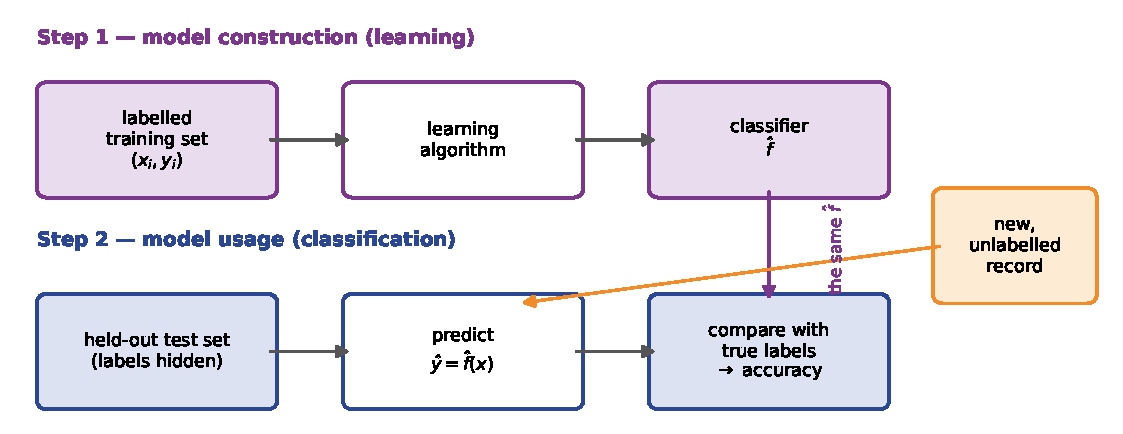
\includegraphics[width=0.86\textwidth]{workflow.pdf}
  \end{center}
  \begin{columns}[T]
    \begin{column}{0.48\textwidth}
      \begin{block}{1. Model construction}
        \small A learning algorithm is given instances whose labels are
        \emph{known} and produces a classifier. Labels supplied $\Rightarrow$
        \textbf{supervised} learning.
      \end{block}
    \end{column}
    \begin{column}{0.48\textwidth}
      \begin{block}{2. Model usage}
        \small Estimate accuracy on an \emph{independent} test set; if it is
        acceptable, label genuinely unknown records.
      \end{block}
    \end{column}
  \end{columns}
  \begin{center}\small
    \textbf{A model that has seen an instance can recite its label, and
    reciting is not predicting.} Two sections from now that becomes a proof.
  \end{center}
\end{frame}

\begin{frame}[fragile,shrink=8]{The whole workflow is three lines}
\begin{lstlisting}
Xtr, Xte, ytr, yte = train_test_split(X, y, test_size=0.3,
                                      random_state=0, stratify=y)
clf = KNeighborsClassifier(n_neighbors=3)   # step 1: construction
clf.fit(Xtr, ytr)
pred = clf.predict(Xte)                     # step 2: usage
\end{lstlisting}
\begin{outblk}
training set (105, 4)  test set (45, 4)
test accuracy 1.0000
confusion matrix (rows = true, cols = predicted)
[[15  0  0]
 [ 0 15  0]
 [ 0  0 15]]
\end{outblk}
\onslide<2->
\begin{alertblock}{Forty-five out of forty-five. Do not be pleased.}
  \footnotesize A clean sweep on $45$ easy test rows is \textbf{not a
  result, it is a small sample} --- and a confusion matrix of zeros teaches
  you nothing about reading one. Score all $150$ rows by cross-validation
  instead.
\end{alertblock}
\end{frame}

\begin{frame}[fragile,shrink=8]{Do it properly: all 150 rows, cross-validated}
\begin{lstlisting}
CV  = StratifiedKFold(5, shuffle=True, random_state=0)   # the one seed
cvp = cross_val_predict(KNeighborsClassifier(3), X, y, cv=CV)
\end{lstlisting}
\begin{outblk}
accuracy 0.9600
confusion matrix (rows = true, cols = predicted)
[[50  0  0]
 [ 0 47  3]
 [ 0  3 47]]
\end{outblk}
\onslide<2->
\begin{alertblock}{Read the matrix, not the number}
  \footnotesize Every \emph{setosa} found --- it is linearly separable from
  the rest. \textbf{All six errors are between \emph{versicolor} and
  \emph{virginica}}, three each way. The single number $0.9600$ hides
  \emph{which} mistake was made --- and in a medical or a credit application,
  the identity of the mistake is the whole question.
\end{alertblock}
\end{frame}

\begin{frame}[fragile,shrink=8]{Precision and recall, from that same matrix}
\begin{outblk}
              precision    recall  f1-score   support

      setosa      1.000     1.000     1.000        50
  versicolor      0.940     0.940     0.940        50
   virginica      0.940     0.940     0.940        50

    accuracy                          0.960       150
   macro avg      0.960     0.960     0.960       150
weighted avg      0.960     0.960     0.960       150
\end{outblk}
\onslide<2->
\begin{columns}[T]
  \begin{column}{0.48\textwidth}
    \begin{block}{Recall of \emph{versicolor} $= 47/50$}
      \small Of the flowers that really \emph{were} versicolor, we found
      $94\%$. Read it \emph{along the row}.
    \end{block}
  \end{column}
  \begin{column}{0.48\textwidth}
    \begin{block}{Precision of \emph{versicolor} $= 47/50$}
      \small Of the flowers we \emph{called} versicolor, $94\%$ really were.
      Read it \emph{down the column}. Equal here only because the errors
      balance.
    \end{block}
  \end{column}
\end{columns}
\begin{center}\small
  A later lecture in this unit builds ROC and AUC on top of this.
  \textbf{Until then: always show the matrix as well as the number.}
\end{center}
\end{frame}

\begin{frame}[shrink=7]{The families of classification algorithm}
  \begin{center}\small
  \begin{tabular}{@{}llp{6.4cm}@{}}
    \toprule
    \textbf{Family} & \textbf{Example} & \textbf{How it draws the boundary}\\
    \midrule
    instance-based & $k$-nearest neighbour & the training points themselves
      define it; no formula \emph{(this lecture)}\\
    linear & logistic regression, linear SVM & one hyperplane
      $w^{\!\top}x + b = 0$\\
    tree-based & ID3, CART & recursive axis-parallel splits\\
    probabilistic & na\"ive Bayes & where the posterior probabilities are
      equal\\
    kernel & SVM with an RBF kernel & a hyperplane in a transformed space\\
    ensemble & bagging, boosting, random forest & many boundaries, combined
      by vote\\
    neural & multi-layer perceptron & composed non-linear maps\\
    \bottomrule
  \end{tabular}
  \end{center}
  \begin{center}\small
    The feature space is $\mathbb{R}^d$; a classifier cuts it into regions,
    one label per region. \textbf{Every algorithm in this unit is a different
    way of drawing the surfaces between those regions.}
  \end{center}
\end{frame}

\begin{frame}[fragile,shrink=8]{Predict first \#1}
\texttt{load\_breast\_cancer}: $569$ patients, $30$ features, five-fold
cross-validation inside a \texttt{Pipeline} with \texttt{StandardScaler}. Six
classifiers, one of which always answers with the commonest class.

\begin{center}
  \textbf{How far apart are the five real classifiers? And where does the
  baseline sit?}
\end{center}
\vspace{0.2em}
\onslide<2->
\begin{outblk}
classifier                     CV acc      std
KNeighborsClassifier(5)        0.9649   0.0215
LogisticRegression             0.9789   0.0142
GaussianNB                     0.9297   0.0124
DecisionTreeClassifier         0.9262   0.0218
SVC(rbf)                       0.9771   0.0070
DummyClassifier                0.6274   0.0039
\end{outblk}
\onslide<3->
\begin{alertblock}{The spread between the five is smaller than the gap to the
baseline}
  \footnotesize Best to worst of the real classifiers: $0.9789$ to $0.9262$,
  about five points. Worst real classifier to \texttt{DummyClassifier}:
  \textbf{thirty points}. \textbf{Choosing the algorithm is usually a smaller
  decision than people expect; choosing the features is usually a larger
  one.} And note $k$-NN is a full point behind logistic regression here.
\end{alertblock}
\end{frame}

\begin{frame}[shrink=8]{Drawn: six classifiers, one dataset}
  \begin{center}
    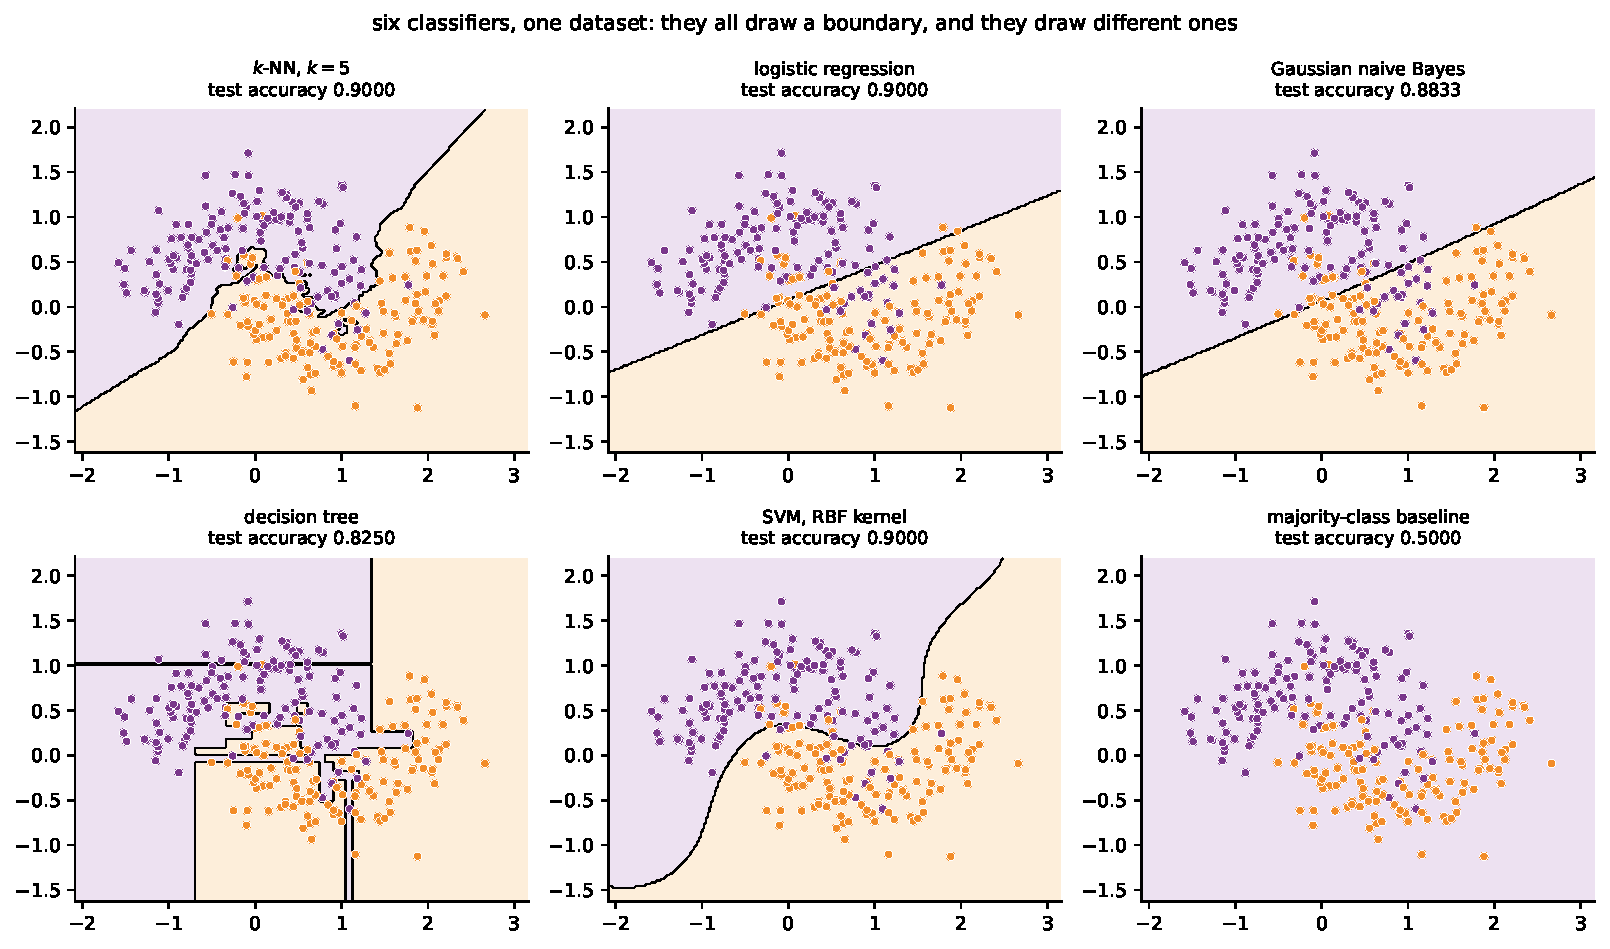
\includegraphics[width=0.84\textwidth]{classifier-landscape.pdf}
  \end{center}
  \begin{center}\small
    The same $280$ training points. Every one of them partitions the plane;
    they disagree about \emph{how}. $k$-NN follows the data, logistic
    regression insists on a straight line, the tree can only cut parallel to
    the axes --- and the baseline paints the whole plane one colour.
  \end{center}
\end{frame}

\begin{frame}[shrink=6]{Eager and lazy: the distinction that organises today}
  \begin{exampleblock}{}
    \centering\small
    An \textbf{eager} learner digests the data into a model at training time
    and then throws the data away. A \textbf{lazy} learner stores the data and
    defers everything until a prediction is demanded.
  \end{exampleblock}
  \begin{center}\small
  \begin{tabular}{@{}lll@{}}
    \toprule
     & \textbf{Eager} & \textbf{Lazy}\\
    \midrule
    training cost & high & essentially zero\\
    prediction cost & low & high, and grows with $n$\\
    memory after training & the model only & the whole training set\\
    what it commits to & one global model & nothing until asked\\
    new training data & usually refit from scratch & append the rows\\
    examples & logistic regression, trees, SVM & $k$-NN, kernel regression\\
    \bottomrule
  \end{tabular}
  \end{center}
  \begin{center}\small
    Lazy learners are also called \textbf{instance-based}, \textbf{memory-based}
    or \emph{non-parametric}. \textbf{``Fitting'' $k$-NN means keeping the
    table.}
  \end{center}
\end{frame}

% =====================================================================
\section[Instance-based]{Instance-based learning, measured}
\label{sec:lazy}

\begin{frame}[fragile,shrink=6]{Cost is cheap to assert. Here it is,
measured}
\texttt{load\_digits}: $1257$ training rows, $540$ test rows, $64$ features.
Best of five repetitions each.
\begin{outblk}
digits: 1257 training rows, 540 test rows, 64 features
model                      fit (ms)   pred (ms)   pred/fit      acc
KNeighborsClassifier(5)       0.234       3.077    13.1455   0.9796
LogisticRegression          844.267       0.101     0.0001   0.9611
DecisionTreeClassifier       10.019       0.079     0.0079   0.8426
GaussianNB                    0.856       0.749     0.8744   0.8481

  KNN  predict: 540 x 1257 distances x 64 features = 43441920 coordinate ops
  KNN  fit    : 0 distances -- it copies 80448 numbers and stops
  LR   predict: 540 x 10 classes x 64 features = 345600 multiply-adds
  LR   fit    : 172 L-BFGS iterations over all 1257 training rows
\end{outblk}
\onslide<2->
\begin{alertblock}{Quote the counts. The milliseconds are this machine only.}
  \footnotesize Per prediction $k$-NN does $\mathbf{125.7\times}$ the
  arithmetic logistic regression does --- exact, on any machine. Its
  \texttt{fit} does \emph{no} distance computations at all. The
  \texttt{pred/fit} column says the same thing with a clock on it: above one
  for $k$-NN, $0.0001$ for logistic regression, a factor of about $10^5$
  apart. \textbf{Timings move between runs on the same machine --- this ratio
  measured between $11$ and $14$. Never read one aloud as a fact.}
\end{alertblock}
\end{frame}

\begin{frame}[shrink=8]{Drawn: a lazy learner pays at prediction time}
  \begin{center}
    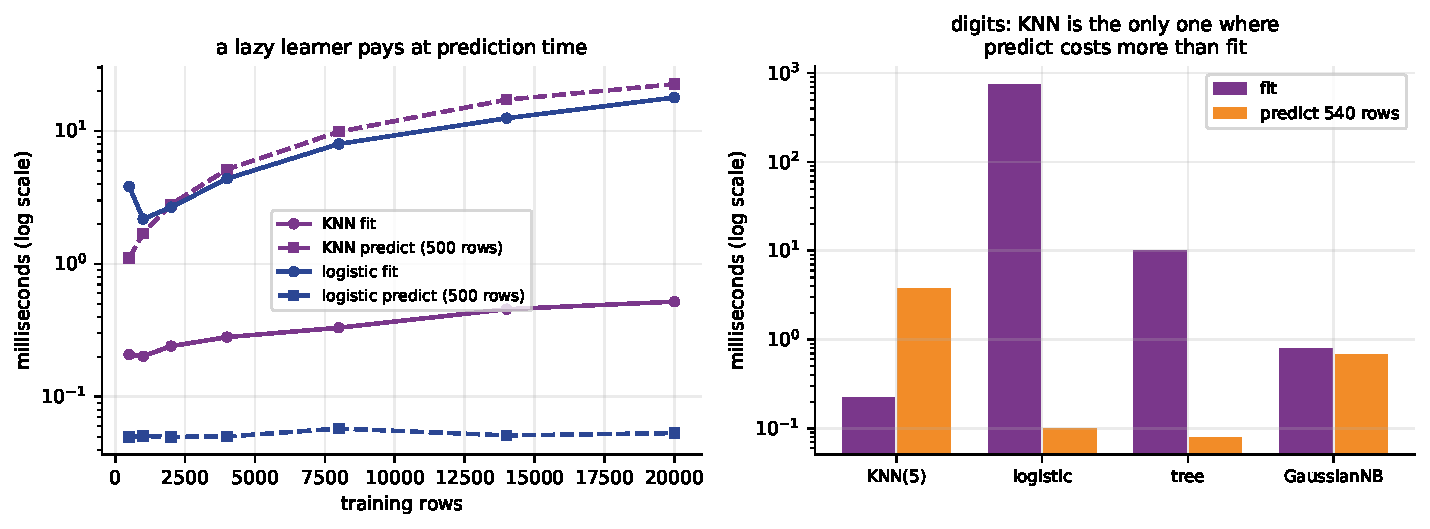
\includegraphics[width=0.86\textwidth]{lazy-vs-eager.pdf}
  \end{center}
  \begin{center}\small
    Left: as the training set grows from $500$ to $20{,}000$ rows, $k$-NN's
    fit time stays flat and its prediction time grows \emph{linearly}, while
    logistic regression does the opposite. Right: the same contrast on
    \texttt{digits}, on a log scale.
  \end{center}
\end{frame}

\begin{frame}[fragile,shrink=6]{Why: $O(nmd)$, and nothing you can do about it}
\begin{columns}[T]
  \begin{column}{0.46\textwidth}
    \begin{block}{\texttt{fit} does one thing}
      \small It copies the training matrix. \texttt{predict} must, for every
      one of $m$ query rows, compute a distance to every one of $n$ stored
      rows over $d$ features: $O(nmd)$.
    \end{block}
  \end{column}
  \begin{column}{0.50\textwidth}
    \begin{alertblock}{So doubling the data doubles the latency}
      \small Not the training time --- the \emph{latency of every answer you
      will ever give}. That is a deployment fact, not a benchmark curiosity.
    \end{alertblock}
  \end{column}
\end{columns}
\vspace{0.2em}
\begin{outblk}
train rows   KNN fit (ms)   KNN predict (ms)   LR fit (ms)   LR pred (ms)   KNN distances
       500          0.206              1.016         2.662         0.061          250000
      2000          0.237              2.702         2.700         0.049         1000000
      8000          0.295              9.921        10.945         0.058         4000000
     20000          0.523             22.039        17.430         0.045       10000000
\end{outblk}
\onslide<2->
\begin{center}\small
  Read the last column. Forty times the training rows is \textbf{exactly}
  forty times the distance computations, $10{,}000{,}000$ against $250{,}000$
  --- true on every machine. The measured time grew by less, and by a
  different factor each run: that gap is BLAS, not mathematics. Logistic
  regression's prediction time did not move at all.
\end{center}
\end{frame}

\begin{frame}[fragile,shrink=6]{And it has to keep the data}
\begin{lstlisting}
kn = KNeighborsClassifier(5).fit(Xdtr, ydtr)
print(kn._fit_X.shape, kn._fit_X.nbytes)
lr = LogisticRegression(max_iter=5000).fit(Xdtr, ydtr)
print(lr.coef_.nbytes + lr.intercept_.nbytes)
\end{lstlisting}
\begin{outblk}
stored training matrix shape (1257, 64)
bytes of training data held   643584
logistic regression stores    5200 bytes, coef_ shape (10, 64)
ratio 123.8 x
\end{outblk}
\onslide<2->
\begin{alertblock}{$k$-NN keeps your training data, and that is a privacy fact}
  \footnotesize An eager model can be shipped without the data it was trained
  on. \textbf{A $k$-NN model \emph{is} the data.} If the training rows are
  patient records or exam scripts, deploying the classifier means deploying
  those records --- and the ratio grows with $n$ while the logistic model's
  size does not. This is not a technicality: it decides whether a model can
  leave the building.
\end{alertblock}
\end{frame}

\begin{frame}[fragile,shrink=8]{Can a KD-tree rescue the prediction cost?}
Partly --- and only in low dimensions. $5000$ points, brute force against a
KD-tree, at three dimensionalities.
\begin{outblk}
features        algo     fit (ms)   predict (ms)   leaves opened per query
2              brute        0.314          9.055
2            kd_tree        1.489         15.361                       1.5
10             brute        0.289         10.742
10           kd_tree        2.767         39.714                      28.6
40             brute        0.287         16.707
40           kd_tree        6.931        169.059                      63.8
\end{outblk}
\onslide<2->
\begin{alertblock}{At $40$ features the tree prunes almost nothing}
  \footnotesize Ignore the clock and read the last column, which is exact.
  At two features a query opens $1.5$ leaves and $6249$ subtrees are thrown
  away unlooked-at. At forty features only $127$ subtrees are pruned in a
  thousand queries and each query opens $63.8$ leaves --- the whole tree. It
  computes every distance brute force would have \emph{and} pays for the
  traversal. \textbf{Leave \texttt{algorithm='auto'} alone; scikit-learn
  already knows this.}
\end{alertblock}
\end{frame}

% =====================================================================
\section[$k$-NN]{$K$-nearest neighbour}
\label{sec:knn}

\begin{frame}[shrink=6]{The entire algorithm}
  \begin{exampleblock}{}
    \centering\small
    To classify a new instance $q$: measure the distance from $q$ to every
    training instance, keep the $k$ closest, and return the commonest label
    among them.
  \end{exampleblock}
  \vspace{0.2em}
  \begin{columns}[T]
    \begin{column}{0.52\textwidth}
      Given $\mathcal{D} = \{(x_i, y_i)\}_{i=1}^{n}$, a distance
      $d(\cdot,\cdot)$ and an integer $k$, let $N_k(q)$ be the $k$ instances
      with smallest $d(q, x_i)$. Then
      \[
        \hat{f}(q) = \arg\max_{c} \sum_{(x_i, y_i) \in N_k(q)}
        \mathbb{1}[y_i = c],
      \]
      with the default distance
      $d(p,q) = \sqrt{\sum_{j} (p_j - q_j)^2}$.
    \end{column}
    \begin{column}{0.44\textwidth}
      \begin{block}{Two examination habits}
        \small \textbf{(1)} Ranking by $d$ and by $d^2$ gives the same order.
        Work in squared distances and take one square root at the end --- or
        none.\\[0.3em]
        \textbf{(2)} $k$ is \emph{not} learned from the data. It is a
        \textbf{hyperparameter}, chosen by validation.
      \end{block}
    \end{column}
  \end{columns}
\end{frame}

\begin{frame}[shrink=8]{By hand: seven points, one query}
Training set: $A(1,1)$, $B(2,2)$, $C(1,3)$ class $0$;
$D(5,4)$, $E(6,5)$, $F(4,7)$ class $1$; and $G(6,2)$ class $0$.
Classify $q_1 = (3,3)$.
\begin{center}\small
\begin{tabular}{@{}lccccccc@{}}
  \toprule
  point & A & B & C & D & E & F & G\\
  \midrule
  $(x_1-3)^2$ & 4 & 1 & 4 & 4 & 9 & 1 & 9\\
  $(x_2-3)^2$ & 4 & 1 & 0 & 1 & 4 & 16 & 1\\
  \midrule
  $d^2$ & 8 & \textbf{2} & 4 & 5 & 13 & 17 & 10\\
  $d$ & 2.8284 & \textbf{1.4142} & 2.0000 & 2.2361 & 3.6056 & 4.1231 &
    3.1623\\
  class & 0 & \textbf{0} & 0 & 1 & 1 & 1 & 0\\
  \bottomrule
\end{tabular}
\end{center}
\begin{center}\small
  Ranked nearest first: \textbf{B, C, D, A, G, E, F}. The nearest neighbour is
  $B$ at $d = \sqrt{2} = 1.4142$, whose class is $\mathbf{0}$.
  \textbf{1-NN predicts class 0.} No square roots were needed to get there.
\end{center}
\end{frame}

\begin{frame}[fragile,shrink=6]{The same thing in code}
\begin{lstlisting}
Xh = np.array([[1,1],[2,2],[1,3],[5,4],[6,5],[4,7],[6,2]], dtype=float)
yh = np.array([0, 0, 0, 1, 1, 1, 0])
knn1 = KNeighborsClassifier(n_neighbors=1).fit(Xh, yh)
dist, idx = knn1.kneighbors(np.array([[3.0, 3.0]]))
\end{lstlisting}
\begin{outblk}
sklearn nearest neighbour index [1] = point B
sklearn distance 1.414214    by hand sqrt(2) = 1.414214
sklearn prediction 0
\end{outblk}
\onslide<2->
\begin{center}\small
  Index $1$ is the second row, which is $B$. The distance agrees with
  $\sqrt{2}$ worked out on paper \textbf{to six decimal places}.
\end{center}
\begin{alertblock}{}
  \centering\small
  There is nothing inside \texttt{KNeighborsClassifier} that you did not just
  do with a pen.
\end{alertblock}
\end{frame}

\begin{frame}[shrink=8]{Drawn: the seven points and the two queries}
  \begin{center}
    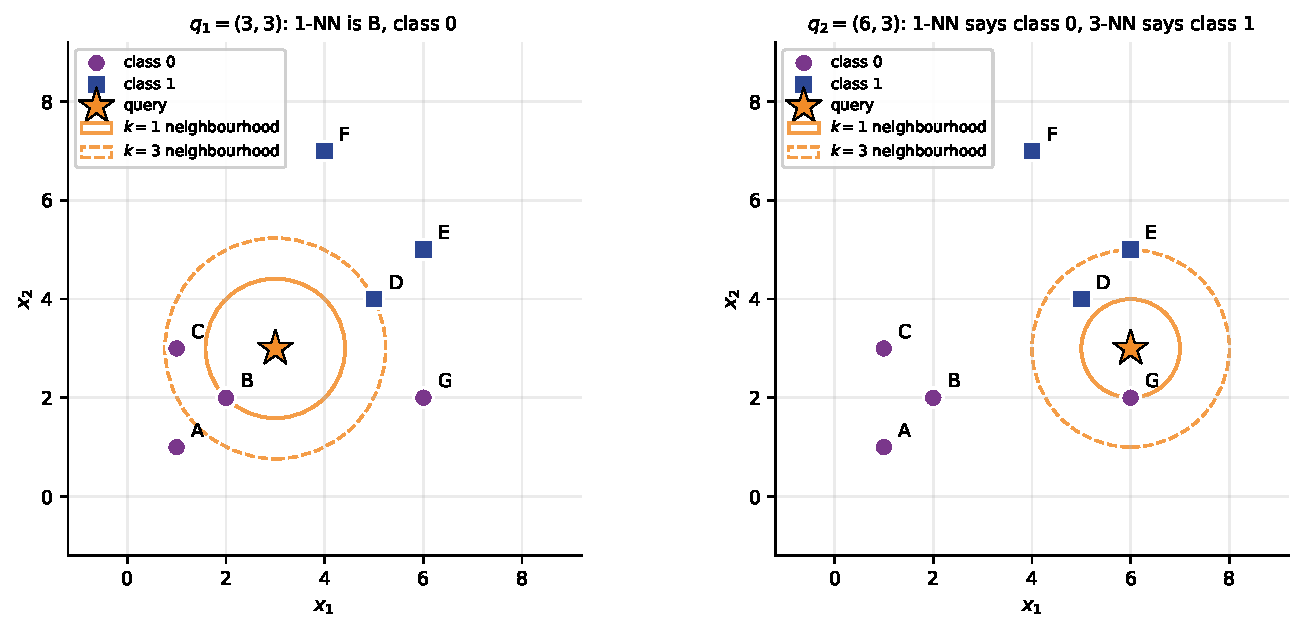
\includegraphics[width=0.80\textwidth]{hand-example.pdf}
  \end{center}
  \begin{center}\small
    The circles have radius equal to the distance to the $1$st and the $3$rd
    nearest neighbour, so \textbf{what falls inside each circle is exactly
    what votes}. Look at $G = (6,2)$: labelled class $0$, but sitting over
    among the class-$1$ points. A mislabelled record, or a genuine oddity.
  \end{center}
\end{frame}

\begin{frame}[shrink=8]{By hand: the query where $k$ changes the answer}
Classify $q_2 = (6, 3)$ --- which lands right next to the odd point $G$.
\begin{columns}[T]
  \begin{column}{0.42\textwidth}
    \begin{center}\small
    \begin{tabular}{@{}lrrrr@{}}
      \toprule
      rank & point & $d^2$ & $d$ & class\\
      \midrule
      1 & G & 1 & 1.0000 & 0\\
      2 & D & 2 & 1.4142 & 1\\
      3 & E & 4 & 2.0000 & 1\\
      4 & B & 17 & 4.1231 & 0\\
      5 & F & 20 & 4.4721 & 1\\
      6 & C & 25 & 5.0000 & 0\\
      7 & A & 29 & 5.3852 & 0\\
      \bottomrule
    \end{tabular}
    \end{center}
  \end{column}
  \begin{column}{0.54\textwidth}
    \begin{block}{Take the vote at four values of $k$}
      \small
      \begin{itemize}
        \item $k=1$: $\{G\}$. Votes $0{:}1$, $1{:}0$ $\to$ \textbf{0}
        \item $k=3$: $\{G,D,E\}$. Votes $0{:}1$, $1{:}2$ $\to$ \textbf{1}
        \item $k=5$: $\{G,D,E,B,F\}$. Votes $0{:}2$, $1{:}3$ $\to$ \textbf{1}
        \item $k=7$: everything. Votes $0{:}4$, $1{:}3$ $\to$ \textbf{0}
      \end{itemize}
    \end{block}
  \end{column}
\end{columns}
\begin{center}\small
  \textbf{Same data, same query, same metric --- four values of $k$, and the
  answer changes twice.}
\end{center}
\end{frame}

\begin{frame}[fragile,shrink=8]{Predict first \#2}
Those four hand-computed votes, run through the library. \textbf{Before the
reveal: what does $k=7$ give, and why is it not a coincidence?}
\vspace{0.2em}
\onslide<2->
\begin{outblk}
k=1  votes  class0=1  class1=0  ->  predict 0   (sklearn 0)
k=3  votes  class0=1  class1=2  ->  predict 1   (sklearn 1)
k=5  votes  class0=2  class1=3  ->  predict 1   (sklearn 1)
k=7  votes  class0=4  class1=3  ->  predict 0   (sklearn 0)
\end{outblk}
\onslide<3->
\begin{columns}[T]
  \begin{column}{0.48\textwidth}
    \begin{block}{Three lessons in one table}
      \footnotesize At $k=1$ a single odd training point dictates the answer.
      At $k=3$ and $k=5$ the vote overrules it --- \emph{that is what averaging
      is for}.
    \end{block}
  \end{column}
  \begin{column}{0.48\textwidth}
    \begin{alertblock}{And at $k=7=n$?}
      \footnotesize The classifier has stopped looking at $q_2$ at all and
      returns the commonest label in the data. \textbf{At $k=n$, $k$-NN
      \emph{is} the majority-class baseline.} Remember that; we cash it in
      twice today.
    \end{alertblock}
  \end{column}
\end{columns}
\end{frame}

\begin{frame}[shrink=8]{1-NN is a Voronoi tessellation}
  \begin{center}
    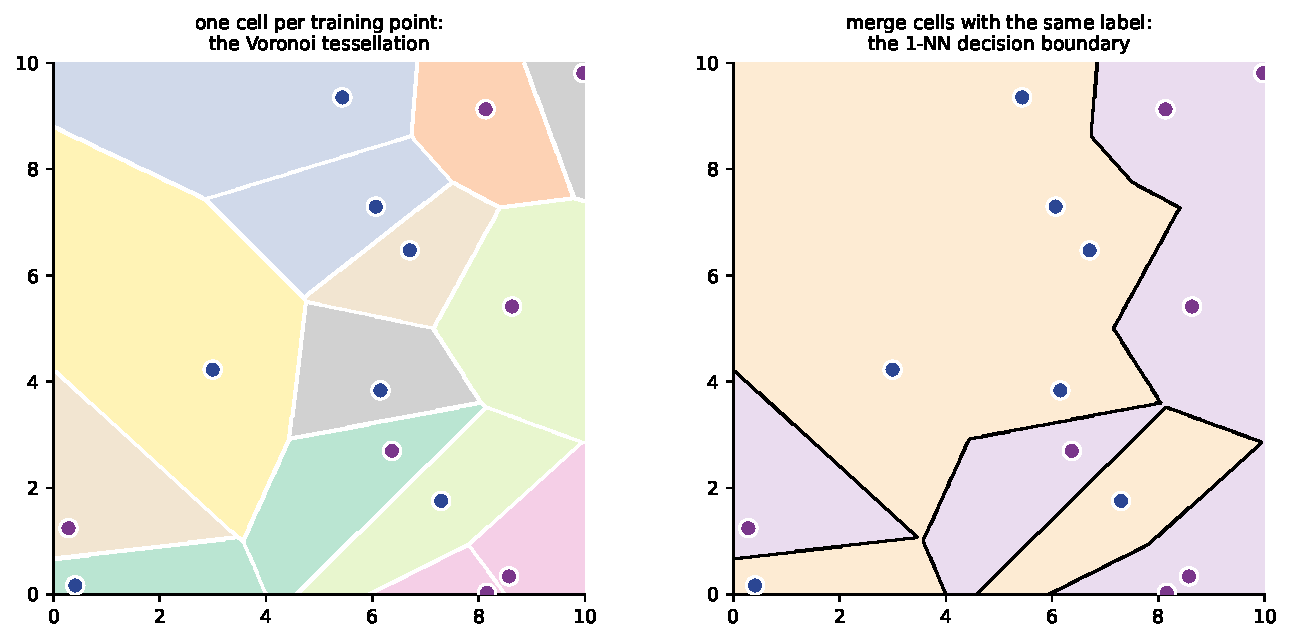
\includegraphics[width=0.76\textwidth]{voronoi.pdf}
  \end{center}
  \begin{center}\small
    Each training point owns everything closer to it than to any other point
    --- its \textbf{Voronoi cell}. Colour each cell by its point's label,
    erase the internal walls, and what remains is the 1-NN decision boundary.
    It is jagged because it is made of \emph{perpendicular bisectors between
    individual data points}: \textbf{move one training point and the boundary
    moves.}
  \end{center}
\end{frame}

% =====================================================================
\section[Choosing $k$]{Choosing $k$}
\label{sec:k}

\begin{frame}[fragile,shrink=6]{$k=1$ memorises --- and here is the proof}
Ask 1-NN about a row that is \emph{in} the training set. The nearest training
point to that row is the row itself, at distance $0$, and its label is the
true label.
\begin{outblk}
nearest neighbour of the first five training rows:
  row 0 -> training row 0 at distance 0.000000
  row 1 -> training row 1 at distance 0.000000
  row 2 -> training row 2 at distance 0.000000
  row 3 -> training row 3 at distance 0.000000
  row 4 -> training row 4 at distance 0.000000
every training row is its own nearest neighbour: True
training accuracy at k=1: 1.000000
\end{outblk}
\onslide<2->
\begin{alertblock}{``My model got 100\% accuracy''}
  \footnotesize Every year somebody reports a perfect $k$-NN score and is
  delighted. \textbf{A training accuracy of $1.0$ at $k=1$ is a consequence of
  arithmetic, not of learning}, it happens on every dataset including one with
  random labels, and it is entirely compatible with the model being useless.
  Quote a cross-validated or held-out score. Always.
\end{alertblock}
\end{frame}

\begin{frame}[fragile,shrink=6]{The gap between training and test accuracy}
Standardised \texttt{breast\_cancer}, a $70/30$ stratified split.
\begin{outblk}
   k   train acc   test acc      gap
   1      1.0000     0.9474    +0.0526
   3      0.9899     0.9415    +0.0484
   5      0.9799     0.9474    +0.0325
  11      0.9774     0.9357    +0.0417
  25      0.9598     0.9415    +0.0183
  51      0.9523     0.9474    +0.0049
 101      0.9271     0.9181    +0.0090
 199      0.8643     0.8538    +0.0105
\end{outblk}
\onslide<2->
\begin{center}\small
  The \texttt{gap} column shrinks as $k$ grows: $+0.0526$ at $k=1$ down to
  $+0.0049$ at $k=51$. A large train-test gap is the signature of
  \textbf{over-fitting}, and in $k$-NN over-fitting is controlled
  \emph{entirely} by $k$. \textbf{Note also that the test column barely
  moves.}
\end{center}
\end{frame}

\begin{frame}[shrink=8]{Drawn: what $k$ does to the boundary}
  \begin{center}
    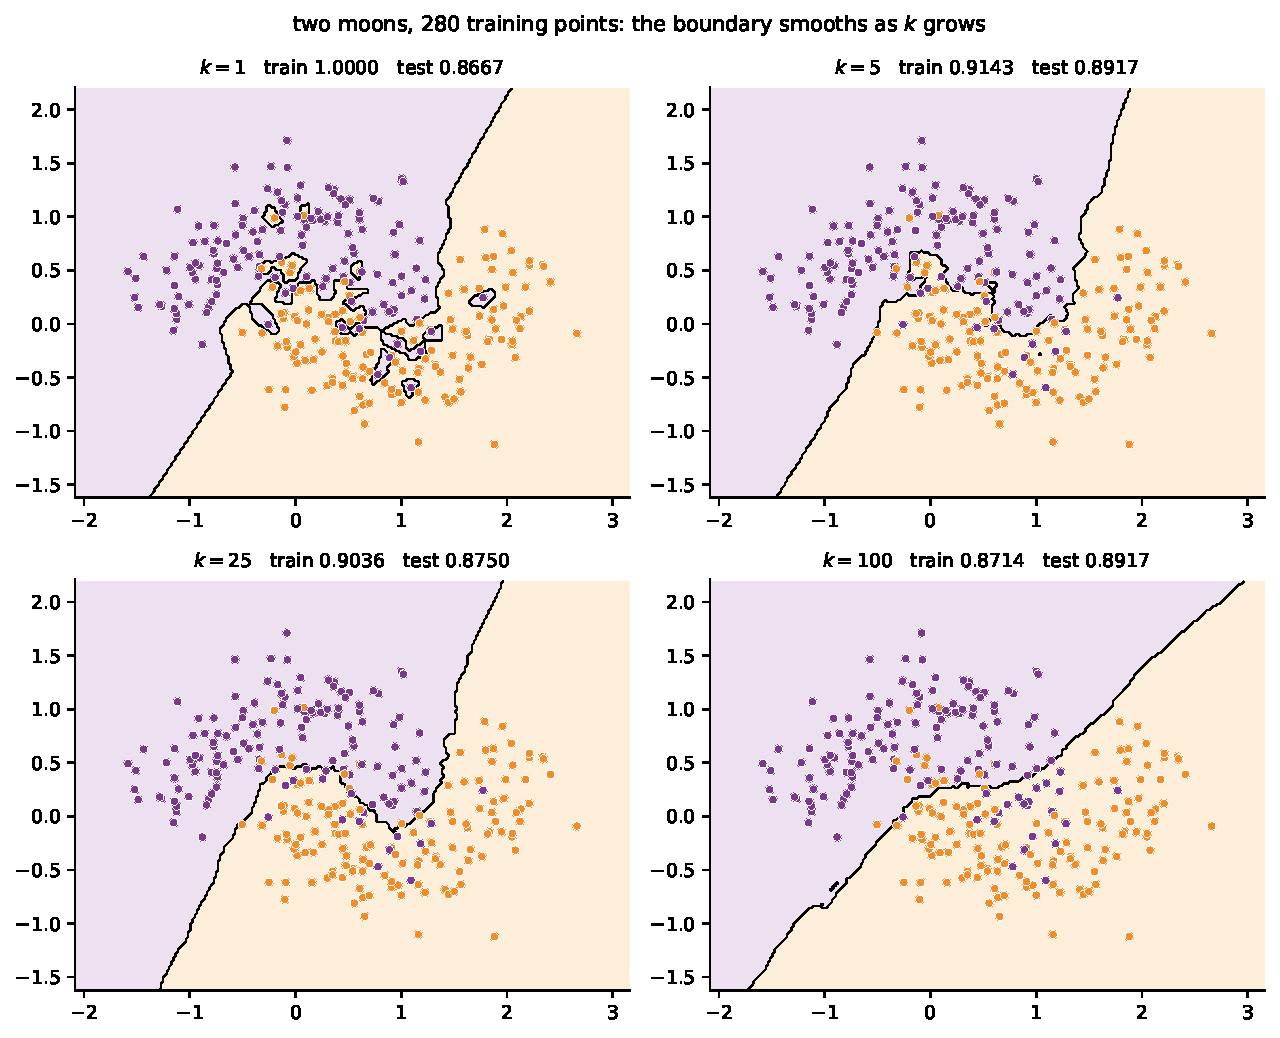
\includegraphics[width=0.62\textwidth]{k-boundaries.pdf}
  \end{center}
  \begin{columns}[T]
    \begin{column}{0.48\textwidth}
      \begin{block}{Small $k$: low bias, high variance}
        \footnotesize Few assumptions; fits any shape, including the shape of
        the noise. Training accuracy $1.0000$ at $k=1$.
      \end{block}
    \end{column}
    \begin{column}{0.48\textwidth}
      \begin{block}{Large $k$: high bias, low variance}
        \footnotesize A smooth, stable boundary that may be too smooth. At
        $k=n$ it is the baseline. Effective parameters $\approx n/k$.
      \end{block}
    \end{column}
  \end{columns}
  \begin{center}\small
    \textbf{Test accuracy across these four panels varies by about one and a
    half points.} The boundary changes far more dramatically than the score
    does.
  \end{center}
\end{frame}

\begin{frame}[fragile,shrink=14]{Predict first \#3}
Standardised \texttt{breast\_cancer} inside a \texttt{Pipeline}, five-fold
cross-validation, $k$ from $1$ to $398$ --- which is $n$ minus the held-out
fold. \textbf{Which $k$ wins, and what \emph{exact} number comes out at
$k=398$?}
\onslide<2->
\begin{outblk}
   k    5-fold CV accuracy      std
   1          0.9578          0.0140
   2          0.9491          0.0217
   3          0.9649          0.0157
   5          0.9649          0.0215
   7          0.9649          0.0192
   9          0.9649          0.0215
  11          0.9666          0.0129
  15          0.9613          0.0106
  21          0.9578          0.0140
  31          0.9543          0.0128
  45          0.9473          0.0123
  65          0.9438          0.0142
  95          0.9297          0.0146
 135          0.9156          0.0204
 199          0.8805          0.0211
 285          0.8015          0.0229
 398          0.6274          0.0039
best k = 11 at CV accuracy 0.9666
majority-class baseline 0.6274
\end{outblk}
\onslide<3->
\begin{center}\small
  \textbf{$0.6274$ was predictable before we ran anything} --- at $k=n$ the
  classifier returns the commonest label, so its accuracy \emph{is} the
  majority-class proportion.
\end{center}
\end{frame}

\begin{frame}[shrink=8]{Drawn: the validation curve is U-shaped}
  \begin{center}
    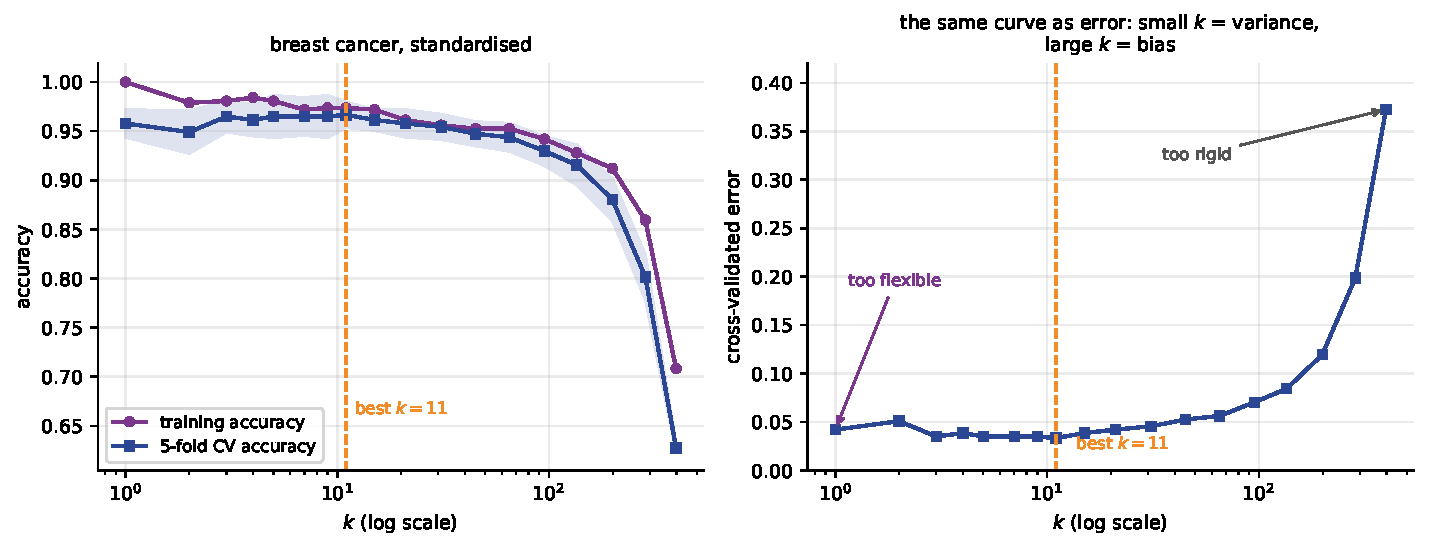
\includegraphics[width=0.82\textwidth]{k-curve.pdf}
  \end{center}
  \begin{columns}[T]
    \begin{column}{0.48\textwidth}
      \begin{block}{Read the right-hand end for free}
        \footnotesize The accuracy at $k=n$ \emph{is} the class balance. A
        free diagnostic on any $k$-NN validation curve. Both ends of the U are
        bad, for opposite reasons.
      \end{block}
    \end{column}
    \begin{column}{0.48\textwidth}
      \begin{alertblock}{And do not over-read the peak}
        \footnotesize $k=3$ to $k=15$ are all within one standard deviation of
        $0.9666$. Report the plateau, not ``the optimal $k$ is $11$'' --- and
        note $k$ was chosen \emph{on these folds}, so $0.9666$ is optimistic.
        \texttt{GridSearchCV} inside an outer split.
      \end{alertblock}
    \end{column}
  \end{columns}
\end{frame}

% =====================================================================
\section[Scaling]{Scaling is not optional}
\label{sec:scale}

\begin{frame}[shrink=8]{By hand: two patients from
\texttt{breast\_cancer}}
$k$-NN's only input is a distance, and a distance is a sum over columns. Take
rows $0$ and $1$, and look at two of their thirty columns.
\begin{center}\small
\begin{tabular}{@{}lrrrr@{}}
  \toprule
  feature & patient 0 & patient 1 & difference & (difference)$^2$\\
  \midrule
  mean area & $1001.0000$ & $1326.0000$ & $-325.0000$ & $105625.0000$\\
  mean smoothness & $0.1184$ & $0.0847$ & $0.0337$ & $0.0011$\\
  \bottomrule
\end{tabular}
\end{center}
\begin{center}\small
  The squared distance over \emph{all thirty} columns is $116779.5720$. So
  \emph{mean area} alone supplies $105625 / 116779.5720 = \mathbf{90.45\%}$
  of it, and \emph{mean smoothness} supplies about
  $\mathbf{0.000001\%}$ --- one part in a hundred million.
\end{center}
\begin{alertblock}{}
  \centering\footnotesize
  Both are real medical measurements. Neither is more important than the
  other. \textbf{The only difference between them is the unit they happen to
  be recorded in.}
\end{alertblock}
\end{frame}

\begin{frame}[fragile,shrink=6]{The same split, computed over all thirty
columns}
\begin{lstlisting}
p, q = bc.data[0], bc.data[1]
tot = ((p - q) ** 2).sum()
share = (p - q) ** 2 / tot
\end{lstlisting}
\begin{outblk}
squared distance over all 30 features 116779.5720
  mean area                contributes  90.4482%
  area error               contributes   5.3876%
  worst area               contributes   3.3987%
  worst perimeter          contributes   0.5700%
the two area columns together contribute 93.8469%
the 27 columns that are not areas contribute 0.7655%
\end{outblk}
\onslide<2->
\begin{alertblock}{Three columns supply $99.23\%$ of the distance}
  \footnotesize The other twenty-seven measurements share $\mathbf{0.7655\%}$
  between them. \textbf{Unscaled $k$-NN on this dataset is a classifier that
  uses three columns and ignores the rest} --- and nothing in its output says
  so.
\end{alertblock}
\end{frame}

\begin{frame}[fragile,shrink=6]{It changes which point is nearest}
\begin{lstlisting}
raw1 = KNeighborsClassifier(1).fit(Xbtr,   ybtr)   # unscaled
std1 = KNeighborsClassifier(1).fit(Xbtr_s, ybtr)   # standardised
n_raw = raw1.kneighbors(Xbte,   return_distance=False)[:, 0]
n_std = std1.kneighbors(Xbte_s, return_distance=False)[:, 0]
\end{lstlisting}
\begin{outblk}
test rows whose nearest neighbour changes when we standardise: 164 of 171
of those, 19 change the predicted class
example: test row 5, true label 1
  raw          nearest is training row 206, label 0
  standardised nearest is training row 69, label 1
\end{outblk}
\onslide<2->
\begin{center}\small
  $164$ of $171$ held-out patients get a \emph{different} nearest neighbour,
  and for $19$ of them the \textbf{answer} changes. Test row $5$ is genuinely
  class $1$; standardising is what gets it right.
\end{center}
\end{frame}

\begin{frame}[shrink=8]{Drawn: the neighbour flips}
  \begin{center}
    
\includegraphics[width=0.90\textwidth]{scaling.pdf}
  \end{center}
  \begin{center}\small
    Left and centre: one held-out patient (star) and its nearest training
    neighbour (circled), on two features, before and after standardising. The
    neighbour changes and so does the predicted class. Right: what
    standardising is worth to a $k=5$ classifier on four bundled datasets ---
    which is the next slide's question.
  \end{center}
\end{frame}

\begin{frame}[fragile,shrink=8]{Predict first \#4}
\texttt{KNeighborsClassifier(5)}, five-fold cross-validation, raw against a
\texttt{StandardScaler} pipeline, on four bundled datasets.

\begin{center}
  \textbf{Rank the four gains. Which is biggest --- and is any of them
  negative?}
\end{center}
\vspace{0.2em}
\onslide<2->
\begin{outblk}
dataset                 raw     scaled      gain
iris                 0.9533     0.9533   +0.0000
wine                 0.6633     0.9608   +0.2975
breast_cancer        0.9315     0.9649   +0.0334
digits               0.9855     0.9766   -0.0089
feature std ratio (widest/narrowest column):
  iris                      4.1
  wine                   2530.3
  breast_cancer        215170.7
\end{outblk}
\onslide<3->
\begin{alertblock}{The size of the scale disparity does \emph{not} predict the
size of the gain}
  \footnotesize \texttt{wine} $+0.2975$ at a ratio of $2530$;
  \texttt{breast\_cancer} only $+0.0334$ at a ratio of $215{,}171$ --- because
  there the dominant area columns happen also to be genuinely informative.
  \texttt{iris}: nothing to fix, all four columns are centimetres.
  \textbf{\texttt{digits}: $-0.0089$ --- scaling made it \emph{worse}},
  because dividing an almost-always-zero border pixel by its tiny standard
  deviation inflates its noise into a full-sized feature.
\end{alertblock}
\end{frame}

\begin{frame}[shrink=6]{So: when to scale, and where to put the scaler}
  \begin{columns}[T]
    \begin{column}{0.48\textwidth}
      \begin{exampleblock}{The rule}
        \small \textbf{Scale when the columns are in different units.} Do not
        scale reflexively when they are already commensurable: standardising a
        near-constant column amplifies its noise. On \texttt{digits} that cost
        $0.0089$ of accuracy.
      \end{exampleblock}
    \end{column}
    \begin{column}{0.48\textwidth}
      \begin{alertblock}{Fit the scaler on the training rows only}
        \small \texttt{StandardScaler} learns a mean and a standard deviation.
        Those are \emph{numbers learned from data}, so the preprocessing rule
        applies unchanged. In practice: put the scaler and the classifier in a
        \texttt{Pipeline} and let \texttt{cross\_val\_score} refit both inside
        every fold.
      \end{alertblock}
    \end{column}
  \end{columns}
  \vspace{0.3em}
  \begin{center}\small
    Thirty points of accuracy on \texttt{wine} for four lines of
    preprocessing. \textbf{No modelling decision in this lecture is worth
    anything like that much.}
  \end{center}
\end{frame}

% =====================================================================
\section[Metrics]{Distance metrics and weighted voting}
\label{sec:metric}

\begin{frame}[shrink=7]{The Minkowski family}
  \[
    d_p(a, b) = \Bigl( \sum_{j=1}^{d} |a_j - b_j|^{p} \Bigr)^{1/p},
    \qquad p \ge 1
  \]
  \begin{center}\small
  \begin{tabular}{@{}llp{6.8cm}@{}}
    \toprule
    $p$ & name & character\\
    \midrule
    $1$ & Manhattan, city-block, $L_1$ & sum of the coordinate differences;
      robust to one large discrepancy\\
    $2$ & Euclidean, $L_2$ & straight-line distance; the default\\
    $p$ & Minkowski-$p$ & \texttt{KNeighborsClassifier(p=...)}\\
    $\infty$ & Chebyshev, $L_\infty$ & the single largest coordinate
      difference\\
    \bottomrule
  \end{tabular}
  \end{center}
  \begin{center}\small
    A diamond for $p=1$, a circle for $p=2$, a square for $p=\infty$.
    \textbf{Changing $p$ changes the shape of ``nearby'', and therefore
    changes who your neighbours are.}
  \end{center}
\end{frame}

\begin{frame}[shrink=8]{By hand: where two metrics disagree}
Query $q = (0,0)$. Two candidates: $P = (3,0)$ of class $0$, and $Q = (2,2)$
of class $1$.
\begin{columns}[T]
  \begin{column}{0.46\textwidth}
    \begin{block}{Manhattan, $p=1$}
      \small $d_1(q,P) = 3 + 0 = 3$\\
      $d_1(q,Q) = 2 + 2 = 4$\\
      Nearest is $P$ $\Rightarrow$ \textbf{class 0}
    \end{block}
    \begin{block}{Euclidean, $p=2$}
      \small $d_2(q,P) = \sqrt{9} = 3$\\
      $d_2(q,Q) = \sqrt{8} = 2.8284$\\
      Nearest is $Q$ $\Rightarrow$ \textbf{class 1}
    \end{block}
  \end{column}
  \begin{column}{0.50\textwidth}
    \begin{exampleblock}{Where does the switch happen?}
      \small Set the two Minkowski distances equal:
      \[
        3 = \bigl(2^p + 2^p\bigr)^{1/p} = 2^{\,1 + 1/p}.
      \]
      Take $\log_2$: $\log_2 3 = 1 + 1/p$, so
      \[
        p^\ast = \frac{1}{\log_2 3 - 1} = 1.709511.
      \]
      Below $p^\ast$: class $0$. Above it: class $1$.
    \end{exampleblock}
  \end{column}
\end{columns}
\begin{center}\small
  \textbf{Same data, same $k$, opposite answers.}
\end{center}
\end{frame}

\begin{frame}[fragile,shrink=8]{The crossover, in code}
\begin{outblk}
p=1         d(q,P)=3.0000   d(q,Q)=4.0000   nearest = P
p=1.5       d(q,P)=3.0000   d(q,Q)=3.1748   nearest = P
p=1.7095    d(q,P)=3.0000   d(q,Q)=3.0000   nearest = P
p=2         d(q,P)=3.0000   d(q,Q)=2.8284   nearest = Q
p=3         d(q,P)=3.0000   d(q,Q)=2.5198   nearest = Q
p=10        d(q,P)=3.0000   d(q,Q)=2.1435   nearest = Q
crossover: 3 = 2^(1+1/p)  gives  p = 1/(log2(3)-1) = 1.709511
Chebyshev (p -> inf): d(q,P)=3.0   d(q,Q)=2.0
\end{outblk}
\onslide<2->
\begin{outblk}
p=1 (manhattan) predicts class 0 for the origin
p=2 (euclidean) predicts class 1 for the origin
\end{outblk}
\onslide<3->
\begin{alertblock}{The metric is part of the model, not an implementation
detail}
  \footnotesize Two $k$-NN classifiers with the \emph{same} $k$ and the
  \emph{same} data are \textbf{different classifiers} if their $p$ differs.
\end{alertblock}
\end{frame}

\begin{frame}[shrink=8]{Drawn: unit balls, the crossover, and three boundaries}
  \begin{columns}[T]
    \begin{column}{0.49\textwidth}
      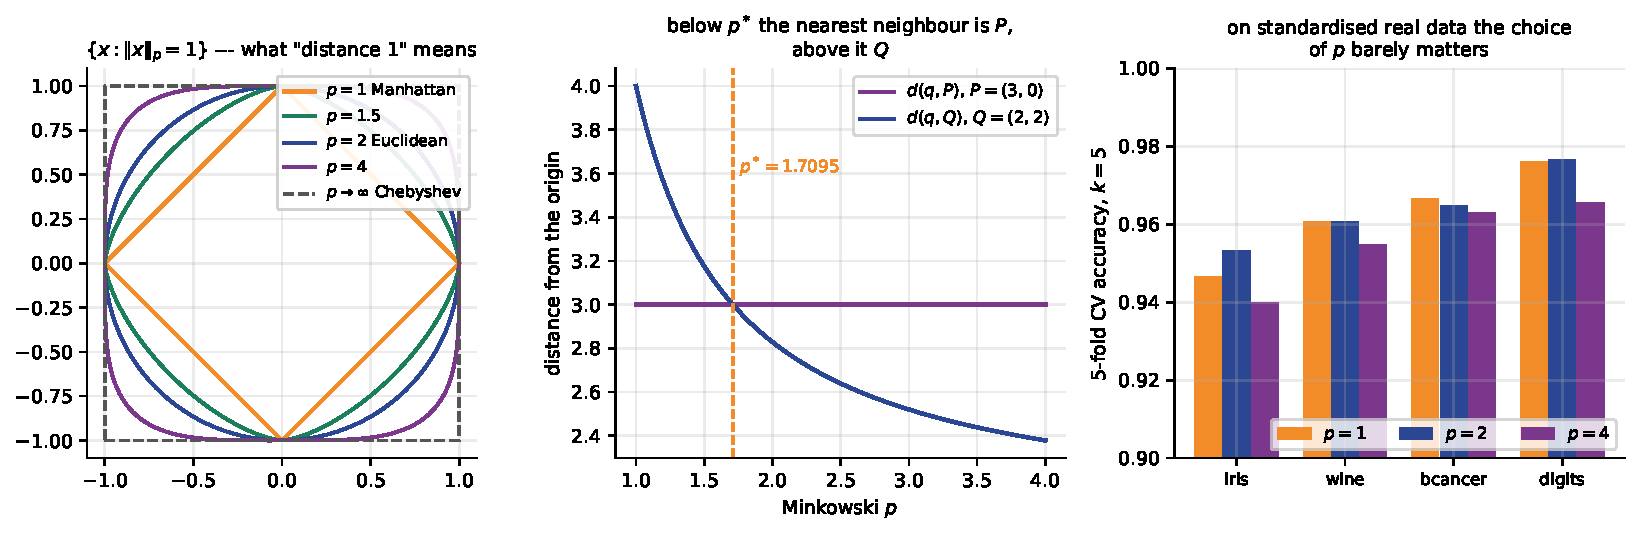
\includegraphics[width=\textwidth]{metrics.pdf}
    \end{column}
    \begin{column}{0.49\textwidth}
      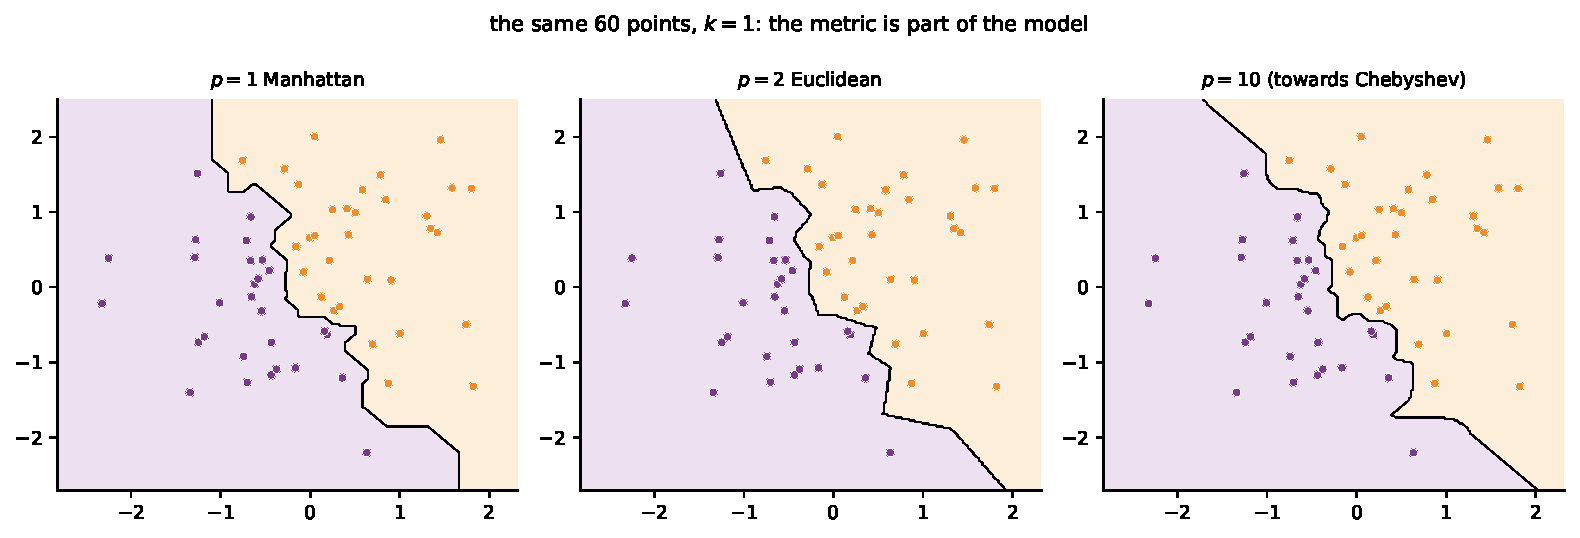
\includegraphics[width=\textwidth]{metric-boundaries.pdf}
    \end{column}
  \end{columns}
  \begin{center}\small
    Left group: the unit balls, the $p^\ast = 1.7095$ crossover, and the
    (small) effect on real data. Right group: the same sixty points at the
    same $k=1$ under three metrics --- Manhattan builds diagonal facets,
    Euclidean builds perpendicular bisectors, near-Chebyshev builds
    axis-aligned steps.
  \end{center}
\end{frame}

\begin{frame}[fragile,shrink=6]{Does $p$ matter in practice? Honestly: not
much}
Four standardised datasets, $k=5$, four metrics.
\begin{outblk}
dataset                p=1       p=2       p=4   chebyshev
iris                0.9467    0.9533    0.9400      0.9400
wine                0.9606    0.9608    0.9549      0.9214
breast_cancer       0.9666    0.9649    0.9631      0.9420
digits              0.9761    0.9766    0.9655      0.9255
\end{outblk}
\onslide<2->
\begin{center}\small
  $p=1$ and $p=2$ are within $0.002$ of each other \emph{everywhere}.
  Chebyshev is consistently the worst, by up to $0.05$ on \texttt{digits},
  because throwing away all but the single largest coordinate difference
  discards most of the information.
\end{center}
\begin{alertblock}{}
  \centering\footnotesize
  Treat $p$ as a hyperparameter worth one line in a grid search --- \textbf{not
  as the place where your accuracy is hiding}. Compare with the $+0.2975$ that
  scaling was worth.
\end{alertblock}
\end{frame}

\begin{frame}[shrink=8]{By hand: distance-weighted voting}
A plain vote treats the nearest neighbour and the $k$th-nearest as equals.
\texttt{weights='distance'} gives each neighbour weight $1/d$.
\begin{center}\small
\begin{tabular}{@{}lrrrrr@{}}
  \toprule
  neighbour & $n_1$ & $n_2$ & $n_3$ & $n_4$ & $n_5$\\
  \midrule
  distance $d$ & $1$ & $2$ & $4$ & $4$ & $5$\\
  label & 1 & 0 & 0 & 0 & 0\\
  weight $1/d$ & $1.0000$ & $0.5000$ & $0.2500$ & $0.2500$ & $0.2000$\\
  \bottomrule
\end{tabular}
\end{center}
\begin{columns}[T]
  \begin{column}{0.48\textwidth}
    \begin{block}{Uniform vote}
      \small Class $0$ gets four, class $1$ gets one. \textbf{Predict 0} ---
      comfortably.
    \end{block}
  \end{column}
  \begin{column}{0.48\textwidth}
    \begin{block}{Weighted vote}
      \small Class $1$: $1.0000$. Class $0$: $0.5 + 0.25 + 0.25 + 0.2 =
      1.2000$. \textbf{Predict 0} --- but only just.
    \end{block}
  \end{column}
\end{columns}
\begin{center}\small
  The margin collapsed from $4{:}1$ to $1.2{:}1.0$. \textbf{Move $n_1$ to
  $d = 0.8$ and its weight becomes $1.25$: the weighted vote flips while the
  uniform vote is unchanged.}
\end{center}
\end{frame}

\begin{frame}[fragile,shrink=8]{Weighted voting: arithmetic, then
measurement}
\begin{outblk}
neighbour distances [1. 2. 4. 4. 5.]
neighbour labels    [1 0 0 0 0]
uniform vote : class1 = 1, class0 = 4  ->  predict 0
weights 1/d         [1.   0.5  0.25 0.25 0.2 ]
distance vote: class1 = 1.0000, class0 = 1.2000  ->  predict 0
\end{outblk}
\onslide<2->
\begin{outblk}
dataset             uniform   distance     gain
iris                 0.9533     0.9533  +0.0000
wine                 0.9665     0.9608  -0.0057
breast_cancer        0.9613     0.9649  +0.0035
digits               0.9622     0.9627  +0.0006
training accuracy of k=25 with distance weights: 1.0000
\end{outblk}
\onslide<3->
\begin{alertblock}{Distance weighting makes \emph{every} $k$ memorise}
  \footnotesize Worth between $-0.0057$ and $+0.0035$ here --- not a free win.
  Its real value: it never produces a tie and it degrades gracefully when $k$
  is too large. But read the last line: at $k=25$ it \textbf{still scores
  $1.0000$ on its own training set}, because a training point is at distance
  $0$ from itself and $1/0$ outvotes everything.
\end{alertblock}
\end{frame}

\begin{frame}[shrink=8]{Drawn: uniform against weighted at $k=15$}
  \begin{center}
    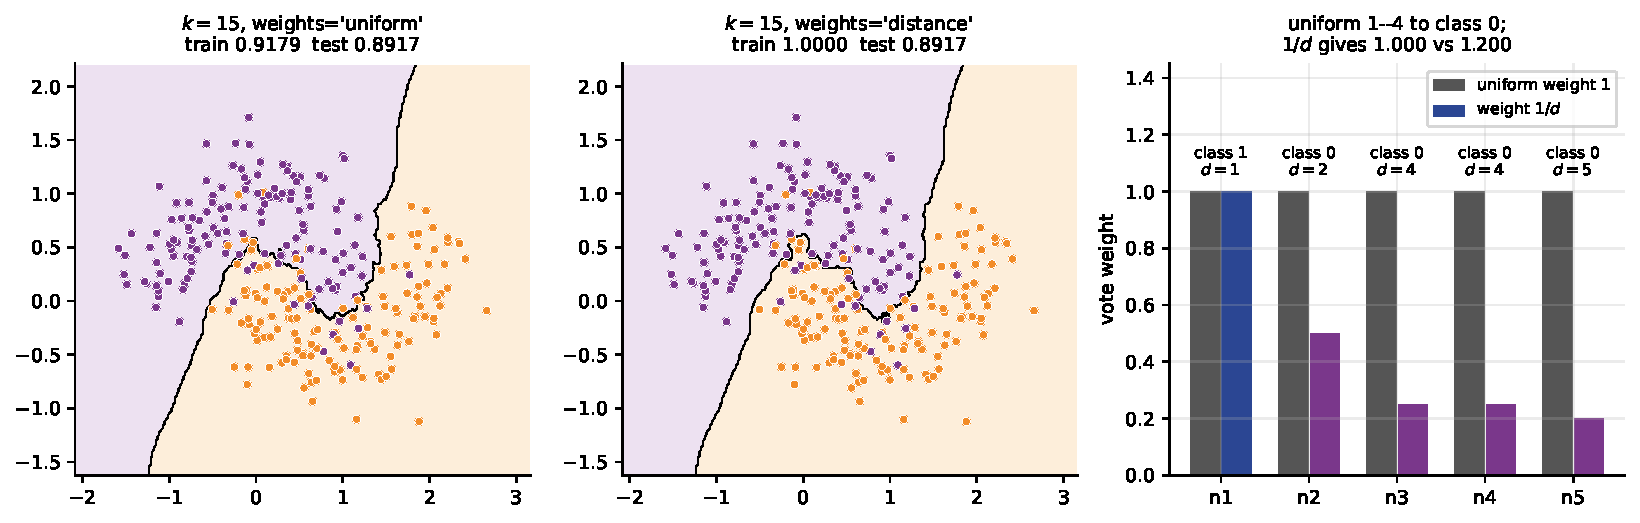
\includegraphics[width=0.90\textwidth]{weighted-voting.pdf}
  \end{center}
  \begin{center}\small
    Left and centre: the same $k=15$, uniform and distance-weighted. The
    weighted version reaches a training accuracy of $1.0000$ \emph{even at
    $k=15$}. Right: the five-neighbour hand calculation, drawn.
  \end{center}
\end{frame}

% =====================================================================
\section[The curse]{The curse of dimensionality}
\label{sec:curse}

\begin{frame}[fragile,shrink=8]{Predict first \#5}
$500$ points drawn uniformly at random in $[0,1]^d$, one query, averaged over
$20$ repetitions. $k$-NN rests on one assumption: that \emph{near} means
something.

\begin{center}
  \textbf{At $d = 1000$, how many times farther away is the farthest point
  than the nearest?}
\end{center}
\vspace{0.2em}
\onslide<2->
\begin{outblk}
   d   mean d_min   mean d_max   d_max/d_min   (max-min)/min
   1       0.0007       0.7705    1156.2859       3577.0046
   2       0.0177       0.9949      56.3273         85.5474
   5       0.1913       1.4461       7.5594          7.0526
  10       0.5743       1.9077       3.3218          2.3636
  20       1.0921       2.4688       2.2605          1.2790
  50       2.1574       3.4987       1.6217          0.6240
 100       3.3890       4.7604       1.4046          0.4053
 500       8.4577       9.7935       1.1579          0.1580
1000      12.2313      13.6006       1.1119          0.1120
\end{outblk}
\onslide<3->
\begin{alertblock}{$\mathbf{1.11\times}$}
  \footnotesize In one dimension the farthest point is over \emph{a thousand
  times} as far away as the nearest. In a thousand dimensions it is $1.11$
  times as far. \textbf{The nearest neighbour is barely nearer than the
  farthest, and a classifier whose whole mechanism is ``find the nearest'' has
  nothing left to work with.}
\end{alertblock}
\end{frame}

\begin{frame}[shrink=8]{Drawn: distances concentrate}
  \begin{center}
    
\includegraphics[width=0.90\textwidth]{curse.pdf}
  \end{center}
  \begin{center}\small
    Left: the ratio $d_{\max}/d_{\min}$ collapses towards $1$. Centre: both
    distances \emph{grow}, and the gap between them stops being a meaningful
    fraction of either. Right: the edge length a neighbourhood must have to
    enclose a fixed fraction of the volume --- which is the next slide.
  \end{center}
\end{frame}

\begin{frame}[fragile,shrink=8]{By hand: how big is a ``small'' neighbourhood?}
Data fill the unit cube $[0,1]^d$ uniformly. You want a cubical neighbourhood
holding $1\%$ of the points. Its volume is $e^d$, so $e^d = 0.01$, that is
$\mathbf{e = 0.01^{1/d}}$.
\begin{outblk}
to capture 1% of the volume of the unit cube, a neighbourhood
must span this fraction of the range of every feature:
  d=   1   0.01^(1/d) = 0.0100
  d=   2   0.01^(1/d) = 0.1000
  d=   5   0.01^(1/d) = 0.3981
  d=  10   0.01^(1/d) = 0.6310
  d=  20   0.01^(1/d) = 0.7943
  d=  50   0.01^(1/d) = 0.9120
  d= 100   0.01^(1/d) = 0.9550
\end{outblk}
\onslide<2->
\begin{alertblock}{In $100$ dimensions that is a box spanning $95.5\%$ of
\emph{every single feature}}
  \footnotesize It is not a neighbourhood; it is nearly the whole dataset.
  \textbf{The word ``local'' has no meaning in high dimensions} --- and $k$-NN
  is a purely local method. Reproduce this argument in the examination; it is
  four lines of arithmetic.
\end{alertblock}
\end{frame}

\begin{frame}[fragile,shrink=6]{The version that will actually happen to you}
Take \texttt{iris}, whose four measurements do a fine job, and bolt on columns
of \emph{pure noise}.
\begin{outblk}
noise cols    KNN(5)     tree   logistic
        0    0.9533   0.9333     0.9600
        2    0.8800   0.9333     0.9400
        5    0.8333   0.9333     0.9667
       10    0.8267   0.9200     0.9400
       25    0.8133   0.9267     0.9333
       50    0.6867   0.9000     0.7600
      100    0.5333   0.9200     0.6800
      200    0.4667   0.9133     0.7000
      400    0.5200   0.9067     0.6067
\end{outblk}
\onslide<2->
\begin{center}\small
  $k$-NN falls from $0.9533$ to $\mathbf{0.5200}$, through a low of $0.4667$
  --- about half its accuracy gone, closing on the one-in-three chance level.
  \emph{Two} noise columns already cost it seven points. The decision tree
  ends at $0.9067$, essentially where it started.
\end{center}
\end{frame}

\begin{frame}[shrink=8]{Drawn: why the tree survives and $k$-NN does not}
  \begin{center}
    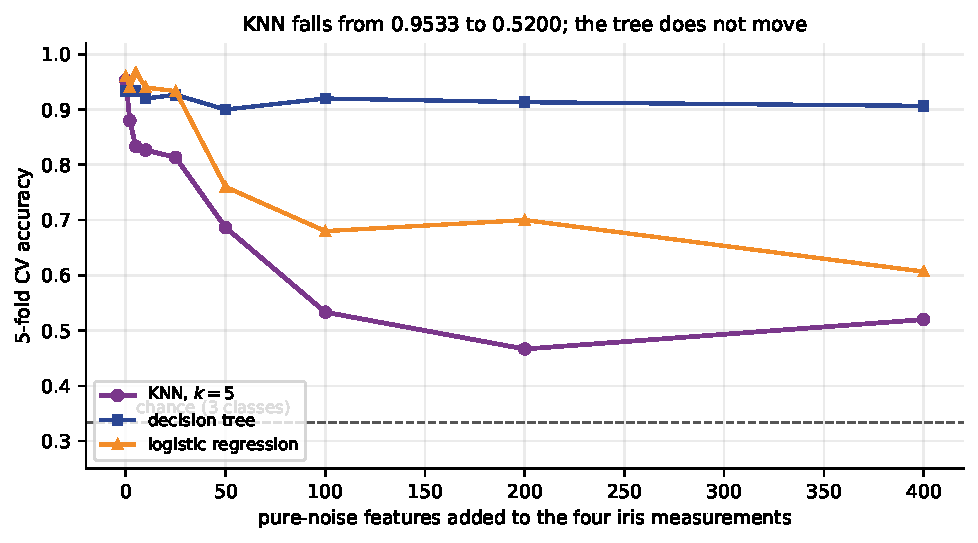
\includegraphics[width=0.58\textwidth]{noise-features.pdf}
  \end{center}
  \begin{alertblock}{$k$-NN has no feature selection built in}
    \footnotesize A decision tree \emph{chooses} which feature to split on and
    can ignore the useless ones. $k$-NN cannot: \textbf{every feature enters
    the distance sum with equal weight, whether or not it carries any
    information}. So before running $k$-NN on a wide table, select features,
    or reduce with PCA, or use a model that selects for you. \textbf{Adding a
    column costs $k$-NN accuracy unless that column earns its place.}
  \end{alertblock}
\end{frame}

% =====================================================================
\section[Failure modes]{Ties, imbalance, and the rest of the failure list}
\label{sec:practical}

\begin{frame}[fragile,shrink=8]{Ties, and how scikit-learn breaks them}
Four points at the corners of a square, labels $0,1,1,0$, query at the exact
centre.
\begin{outblk}
all four neighbours at distance [1.4142 1.4142 1.4142 1.4142]
their labels [0 1 1 0]
k=4 probabilities [0.5 0.5] -> predict 0
k=2 probabilities [0.5 0.5] -> predict 0
k=3 probabilities [0.33333333 0.66666667] -> predict 1
\end{outblk}
\onslide<2->
\begin{columns}[T]
  \begin{column}{0.49\textwidth}
    \begin{alertblock}{Deterministically, towards the smaller label}
      \footnotesize It takes the \texttt{argmax} of the vote counts, which
      returns the \emph{first} maximum. \textbf{It does not toss a coin and it
      does not warn you.}
    \end{alertblock}
  \end{column}
  \begin{column}{0.49\textwidth}
    \begin{block}{Three consequences}
      \footnotesize \textbf{(1)} Use an odd $k$ for two classes --- $k=2$
      scored $0.9491$, below both $k=1$ and $k=3$. \textbf{(2)} An odd $k$
      does \emph{not} help with three or more classes: $3{:}3{:}3$ at $k=9$.
      \textbf{(3)} Distance ties are broken by row order, so reordering the
      training rows can change the prediction.
    \end{block}
  \end{column}
\end{columns}
\end{frame}

\begin{frame}[fragile,shrink=6]{Imbalanced classes: the most important table
today}
$2000$ rows, a $94{:}6$ split, ten features.
\begin{outblk}
class counts [1882  118]
   k   accuracy   minority recall   minority predicted
   1     0.9367            0.4000               31
   3     0.9483            0.2571               14
   5     0.9550            0.2571               10
  15     0.9417            0.0000                0
  51     0.9417            0.0000                0
 151     0.9417            0.0000                0
always predicting the majority class scores 0.9417
k=51 with distance weights: accuracy 0.9417, minority recall 0.0000
\end{outblk}
\onslide<2->
\begin{alertblock}{$0.9417$ and $0.0000$ describe the same classifier}
  \footnotesize At $k \ge 15$ it predicts the minority class \textbf{zero
  times} on $600$ held-out rows and scores exactly the baseline. The mechanism
  is arithmetic: at $6\%$ minority, a neighbourhood of $51$ contains about $3$
  minority points and needs $26$ to win. \textbf{Never report accuracy alone
  on imbalanced data.}
\end{alertblock}
\end{frame}

\begin{frame}[shrink=8]{Drawn: accuracy hides it completely}
  \begin{center}
    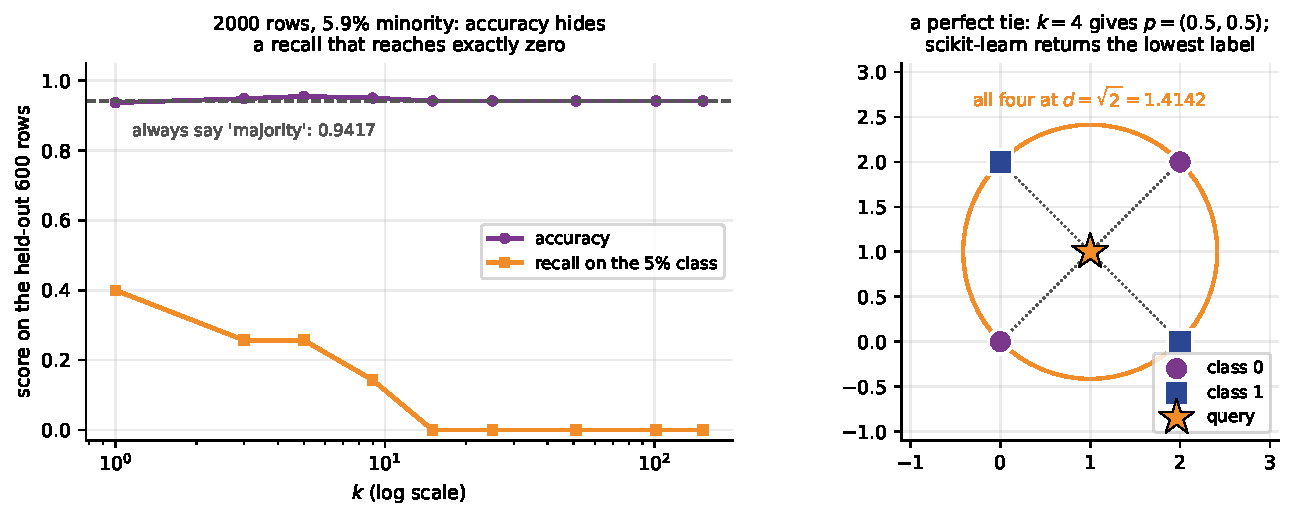
\includegraphics[width=0.90\textwidth]{imbalance-and-ties.pdf}
  \end{center}
  \begin{center}\small
    Left: accuracy stays around $0.94$ for every $k$ while minority recall
    falls to \emph{exactly zero}. Right: the four-way distance tie. Three
    fixes, in order of preference: \textbf{resample} the training set; use
    \texttt{predict\_proba} with a threshold below $0.5$; or choose an
    algorithm supporting \texttt{class\_weight='balanced'} --- which
    \texttt{KNeighborsClassifier}, note, does \emph{not}.
  \end{center}
\end{frame}

\begin{frame}[shrink=9]{The complete failure list --- and why we teach it
anyway}
\begin{columns}[T]
  \begin{column}{0.60\textwidth}
    \begin{center}\tiny
    \begin{tabular}{@{}p{2.5cm}p{2.4cm}p{2.7cm}@{}}
      \toprule
      \textbf{Failure} & \textbf{Symptom} & \textbf{Fix}\\
      \midrule
      unscaled features & one column supplies $90\%$ of the distance &
        \texttt{StandardScaler} in a \texttt{Pipeline}\\
      $k$ too small & training $1.0$, test much lower & raise $k$;
        cross-validate\\
      $k$ too large & accuracy equals the baseline & lower $k$\\
      even $k$, two classes & silent tie-breaking & odd $k$, or
        \texttt{weights='distance'}\\
      irrelevant features & accuracy falls as columns are added &
        feature selection, or PCA\\
      high dimension & all distances nearly equal & reduce $d$; another
        algorithm\\
      imbalanced classes & minority recall $0$, accuracy high & resample;
        move the threshold\\
      slow prediction & latency grows with $n$ & index in low $d$; an eager
        learner\\
      large model & the training data ships with the model & an eager
        learner\\
      missing values & \texttt{nan} poisons every distance & impute before
        fitting\\
      categorical features & ``distance'' between two words & encode, or a
        mixed metric\\
      \bottomrule
    \end{tabular}
    \end{center}
  \end{column}
  \begin{column}{0.38\textwidth}
    \begin{exampleblock}{Four reasons it survives}
      \footnotesize
      \begin{enumerate}
        \item \textbf{The honest baseline.} One hyperparameter, no
          assumptions. If your elaborate model cannot beat it, it is not
          earning its keep.
        \item \textbf{No assumption about the boundary.} Cover--Hart:
          asymptotically 1-NN's error is at most twice the best possible.
        \item \textbf{Naturally multi-class.} On \texttt{digits} it scored
          $0.9796$ against logistic regression's $0.9611$.
        \item \textbf{It needs no feature vector} --- only a distance. Edit
          distance, dynamic time warping, graph distance.
      \end{enumerate}
    \end{exampleblock}
  \end{column}
\end{columns}
\end{frame}

% =====================================================================
\section{Summary}
\label{sec:summary}

\begin{frame}[shrink=16]{Summary --- fourteen lines}
  \begin{enumerate}\small
    \item Classification predicts a label from a finite set. Han, Kamber and
      Pei's general approach has two steps: \textbf{model construction}, then
      \textbf{model usage} with accuracy estimated on an independent test set.
    \item Read the confusion matrix, not the accuracy. One $70/30$ split of
      iris scored $1.0000$ and said nothing; cross-validated over all $150$
      rows the score was $0.9600$ and \emph{every} error was between
      \emph{versicolor} and \emph{virginica}.
    \item The spread between five real classifiers on breast\_cancer
      ($0.9262$ to $0.9789$) is smaller than the gap from the worst of them to
      the $0.6274$ baseline.
    \item \textbf{Eager} works at fit time; \textbf{lazy} works at predict
      time. On \texttt{digits} $k$-NN does $125.7\times$ the arithmetic per
      prediction; the predict/fit ratio is above $1$ for $k$-NN and
      $0.0001$ for logistic regression --- a factor of $10^{5}$.
    \item A fitted $k$-NN \emph{is} the data: $643{,}584$ bytes against
      $5{,}200$, and $40\times$ the rows is exactly $40\times$ the distances.
    \item The algorithm: distance to every point, keep the $k$ smallest, vote.
      By hand, $1$-NN put $q_1 = (3,3)$ in class $0$ via $B$ at $d=\sqrt{2}$
      --- and the library returned $1.414214$.
    \item $k$ changes the answer: on $q_2 = (6,3)$, $k=1 \to 0$,
      $k=3 \to 1$, $k=5 \to 1$, $k=7 \to 0$. \textbf{At $k = n$ it is the
      majority-class baseline.}
    \item \textbf{$k=1$ scores exactly $1.000000$ on its own training set},
      because every row is its own nearest neighbour at distance $0$. Training
      accuracy is worthless evidence here.
    \item The validation curve peaked at $k=11$ with $0.9666$ and fell to
      $0.6274$ at $k=398$. The peak is \textbf{shallow}: $k=3$ to $k=15$ are
      indistinguishable.
    \item \textbf{Scaling.} \emph{Mean area} alone supplied $90.4482\%$ of one
      squared distance; the $27$ non-area columns shared $0.7655\%$.
      Standardising changed the nearest neighbour of $164$ of $171$ test
      patients and the class of $19$.
    \item Gains at $k=5$: \texttt{wine} $+0.2975$, \texttt{breast\_cancer}
      $+0.0334$, \texttt{iris} $+0.0000$, \texttt{digits}
      $\mathbf{-0.0089}$. Scale when the units differ, not reflexively.
    \item Minkowski: $P$ wins under $L_1$, $Q$ under $L_2$, crossover at
      $p^\ast = 1.7095$. On real data $p$ moves accuracy by under $0.01$;
      distance weighting by between $-0.0057$ and $+0.0035$ --- and it makes
      \emph{every} $k$ score $1.0$ on the training set.
    \item \textbf{The curse.} $d_{\max}/d_{\min}$ is $1156$ at $d=1$ and
      $1.11$ at $d=1000$. A box holding $1\%$ of the data in $100$ dimensions
      spans $95.5\%$ of every feature. Adding noise columns to iris took
      $k$-NN from $0.9533$ to $0.5200$; the tree went $0.9333$ to $0.9067$.
    \item On a $94{:}6$ problem, $k \ge 15$ predicted the minority class zero
      times in $600$ rows while scoring $0.9417$ --- exactly the baseline.
      \textbf{Never report accuracy alone.}
  \end{enumerate}
\end{frame}

\begin{frame}[shrink=3]{Before the next lecture}
  \begin{columns}[T]
    \begin{column}{0.48\textwidth}
      \begin{block}{Read}
        \texttt{notes.pdf} --- the full development, the Voronoi argument, the
        complete failure table, and \textbf{10 practice questions with worked
        solutions}.
      \end{block}
      \begin{block}{Do}
        Questions 1, 2 and 5, \textbf{with a pen}. Question 1 is a distance
        table and three values of $k$; question 5 is a Minkowski crossover you
        must derive, not guess.
      \end{block}
    \end{column}
    \begin{column}{0.48\textwidth}
      \begin{exampleblock}{Next: decision trees}
        Attribute selection measures, information gain, ID3, and turning a
        tree into rules. Carry one contrast across: \textbf{$k$-NN weights
        every column equally; a tree chooses.} That single sentence explains
        the last figure of this lecture.
      \end{exampleblock}
      \begin{alertblock}{And a habit to start now}
        Every $k$-NN you write goes in a \texttt{Pipeline} with a scaler, and
        every score you quote is cross-validated. If you catch yourself
        reporting \texttt{score(Xtr, ytr)}, stop.
      \end{alertblock}
    \end{column}
  \end{columns}
  \begin{center}
    \small Materials: \texttt{\AMLRepoURL}
  \end{center}
  \slidesources{\AMLUnitVISources}
\end{frame}

\end{document}
